\documentclass[../../main.tex]{subfiles}

\begin{document}
\section{No Power-Law Behavior in Hidden Markov Models}
    \label{section:no_power-law_in_hidden_markov_models}
    When modelling \emph{natural language}, we generate the next token(s) based on the previous tokens (and hence not based on future tokens; we generate text from left to right). Thus, when disregarding the future tokens, i.e. when marginalizing over them, we can determine the Markov blanket of the current token, i.e. determine the minimal set of tokens that influence the current one.

    Naturally, we can think of natural language modelling as \emph{Bayesian networks} over the characters in the text. Because we generate text from left to right, we naturally assume all arrows to go from previous tokens to future tokens (because this is also the modus operandi for token generation). For example, Markov chains up to character position $t$ have the following simple representation:

    \begin{figure}[h]
        \center
        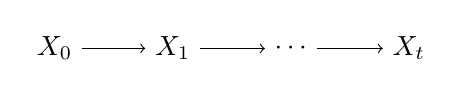
\begin{tikzpicture}[node distance=1.5cm, auto]
        \node (X0) {$X_0$};
        \node (X1) [right of=X0] {$X_1$};
        \node (dots) [right of=X1] {$\cdots$};
        \node (Xt) [right of=dots] {$X_t$};

        \draw[->] (X0) -- (X1);
        \draw[->] (X1) -- (dots);
        \draw[->] (dots) -- (Xt);
        \end{tikzpicture}
        \caption{Bayesian network of Markov chains. All arrows go from previous tokens to future tokens.}
        \label{fig:bayesian_network_markov_chain}
    \end{figure}

    But really, in time-homogenous Markov chains $P(X_{t + 1} = a \mid X_t = b)$ is independent of $t$ and hence is constant over time. Thus, all the arrows in figure~\ref{fig:bayesian_network_markov_chain} represent the same transition.

    From a modelling perspective, it is very reasonable to reuse the same transitions over time, as we cannot have infinitely many "hard-coded" transitions (but we can use different models with implicitly infinite transitions). Furthermore, when making a prediction of the next token given a fixed context window, it seems reasonable to assume invariance in time, i.e. fixed transition probabilities similar to time-homogenous Markov chains.

    Now, the question is, can we achieve power-law behavior with an arbitrarily large fixed-sized context window with fixed transition probabilities?

    In order to answer this question, let us first reduce our setting to a simpler model, specifically to the already mentioned time-homogenous Markov chains:
    
    The idea is to employ a hidden variable $Y \in \Sigma ^{s+1}$, where $\Sigma$ is the alphabet, and $s$ is the size of the context window (for Markov chains $s = 1$). Clearly, $Y$ captures the entire \emph{state} at time $t$ of our model, that is all the previous $s$ tokens and the current one, and we can model the transitions $Y_t \to Y_{t + 1}$ as simple time-homogenous Markov chain transitions (and hence invariant in time). And, of course, once we know $Y_t$, we also know $X_t$ (which of course can be modelled with time-homogenous Markov chain transitions as well). These models are known as \emph{hidden Markov models}.

    \begin{figure}[h]
        \center
        \begin{tikzpicture}[node distance=1.5cm and 1.5cm, auto]

        % Top row (Y)
        \node (Y0) {$Y_0$};
        \node (Y1) [right of=Y0] {$Y_1$};
        \node (Ydots) [right of=Y1] {$\cdots$};
        \node (Yt) [right of=Ydots] {$Y_t$};

        % Bottom row (X)
        \node (X0) [below of=Y0] {$X_0$};
        \node (X1) [right of=X0] {$X_1$};
        \node (Xdots) [right of=X1] {$\cdots$};
        \node (Xt) [right of=Xdots] {$X_t$};

        % Horizontal arrows (Y row)
        \draw[->] (Y0) -- (Y1);
        \draw[->] (Y1) -- (Ydots);
        \draw[->] (Ydots) -- (Yt);

        % Vertical arrows
        \draw[->] (Y0) -- (X0);
        \draw[->] (Y1) -- (X1);
        \draw[->] (Yt) -- (Xt);

        \end{tikzpicture}
        \caption{Bayesian network of a hidden Markov model.}
        \label{fig:bayesian_network_hidden_markov}
    \end{figure}

    \bigskip
    Unfortunately, there is no free lunch, as we will see in the following. However, in order to use theorem \ref{theorem:power_law_decay_in_well-behaved_models_with_weak_power-law_behavior} to disprove weak and thus strong power-law behavior, we need to prove the bulk marginal property of hidden Markov models first:
 
    \begin{lemma}[Hidden Markov Models have the Bulk Marginal Property]
        Every hidden Markov model with finite state spaces $(S_Y, S_X)$ for its latent variable $Y$ and observable variable $X$ with transition matrices $(\bm{M_Y}, \bm{M_X})$ complies with the bulk marginal property.
    \end{lemma}
    \vspace{-2.5em}
    \begin{proof}
        Let $w_i \coloneqq X_{i - 1}$ for $n \in [n + 1]$. Then we have:
        \begin{align*}
            &\sum_{w_{n + 1} \in \Sigma} S_{n + 1}(w) \\
            &\underset{\text{Bayesian network}}{=} \sum_{w_{n + 1} \in \Sigma} \sum_{q_1, \dots, q_{n+1} \in S_Y} \left[ P(q_1) \prod_{i=2}^{n+1} P(q_i \mid q_{i-1}) \cdot \prod_{i=1}^{n+1} P(w_i \mid q_i) \right] \\
            &= \sum_{q_1, \dots, q_{n+1} \in S_Y} \sum_{w_{n + 1} \in \Sigma}  \left[ P(q_1) \prod_{i=2}^{n+1} P(q_i \mid q_{i-1}) \cdot \prod_{i=1}^{n+1} P(w_i \mid q_i) \right] \\
            &= \sum_{q_1, \dots, q_{n+1} \in S_Y} \left[ P(q_1) \prod_{i=2}^{n+1} P(q_i \mid q_{i-1}) \cdot \prod_{i=1}^{n} P(w_i \mid q_i) \sum_{w_{n + 1} \in \Sigma}  P(w_{n+1} \mid q_{n+1}) \right] \\
            &= \sum_{q_1, \dots, q_{n+1} \in S_Y} \left[ P(q_1) \prod_{i=2}^{n+1} P(q_i \mid q_{i-1}) \cdot \prod_{i=1}^{n} P(w_i \mid q_i) \right] \\
            &= \sum_{q_1, \dots, q_{n} \in S_Y} \sum_{q_{n+1} \in S_Y} P(q_{n+1} \mid q_n) \left[ P(q_1) \prod_{i=2}^{n} P(q_i \mid q_{i-1}) \cdot \prod_{i=1}^{n} P(w_i \mid q_i) \right] \\
            &= \sum_{q_1, \dots, q_{n} \in S_Y} \left[ P(q_1) \prod_{i=2}^{n} P(q_i \mid q_{i-1}) \cdot \prod_{i=1}^{n} P(w_i \mid q_i) \sum_{q_{n+1} \in S_Y} P(q_{n+1} \mid q_n) \right] \\
            &= \sum_{q_1, \dots, q_{n} \in S_Y} \left[ P(q_1) \prod_{i=2}^{n} P(q_i \mid q_{i-1}) \cdot \prod_{i=1}^{n} P(w_i \mid q_i) \right] \\
            &\overset{\checkmark}{=} S_n(w_{-\{n+1\}}) \quad .
        \end{align*}
    \end{proof}

    We will also make use of the following well-established results regarding time-homogenous Markov chains. Hence, they are stated without proof:

      \begin{lemma}
        \label{lemma:raising_marov_matrix_to_its_period}
        Let $\bm{M}$ be the transition matrix for an irreducible Markov chain with period $p$. Then the chain described by $\bm{M}^p$ consists of exactly $p$ aperiodic, closed communication classes.
    \end{lemma}

    \begin{lemma}
        \label{lemma:irreducible_aperiodic_markov_chain_stays_irreducible_aperiodic}
        Let $\bm{M}$ describe an irreducible aperiodic Markov chain. Then, for every $n \in \mathbb{N}_{>0}$, the Markov chain described by $\bm{M}^n$ is also irreducible and aperiodic.
    \end{lemma}

    Additional prerequisites can be found in the appendix, see section~\ref{section:prerequisites_for_theorem}.

    With all that being covered, we can finally state and prove our main result:

    \begin{theorem}[No Hidden Markov Model with Power-Law Behavior]
        \label{theorem:no_hidden_markov_model_with_power-law}
        % There is no hidden Markov model $(\bm{M_Y}, \bm{M_X})$ with $I(X_{t_0}, X_{t_0 + \tau}) \in \mathcal{O}(\tau^{-\alpha})$ and $I(X_{t_0}, X_{t_0 + \tau}) \in \Omega (\tau^{-\beta})$ for some $\alpha, \beta \in \mathbb{R}_{>0}$.
        There is no hidden Markov model $(\bm{M_Y}, \bm{M_X})$ with with weak power-law behavior (and hence also strong power-law behavior).
    \end{theorem}
    \vspace{-2.5em}
    \begin{proof}
        Since hidden Markov models satisfy the bulk marginal property, we can use the contraposition of theorem~\ref{theorem:power_law_decay_in_well-behaved_models_with_weak_power-law_behavior} to show that hidden Markov models are incapable of weak power-law behavior. Note that we can choose our starting referencing random variable freely. Hence, we may analyze $I(X_0; X_{\tau})$.

        First, note that we can construct the following Bayesian network with adjusted transitions depicted in figure~\ref{fig:adjusted_bayesian_network_hidden_markov}.

        \begin{figure}[h]
            \center
            \begin{tikzpicture}[node distance=1.5cm and 1.5cm, auto]

            % Top row (Y)
            \node (Y0) {$Y_0$};
            \node (Y1) [right of=Y0] {$Y_1$};
            \node (Ydots) [right of=Y1] {$\cdots$};
            \node (Yt) [right of=Ydots] {$Y_\tau$};

            % Bottom row (X)
            \node (X0) [below of=Y0] {$X_0$};
            \node (X1) [right of=X0] {$X_1$};
            \node (Xdots) [right of=X1] {$\cdots$};
            \node (Xt) [right of=Xdots] {$X_\tau$};

            % Horizontal arrows (Y row)
            \draw[->] (Y0) -- (Y1);
            \draw[->] (Y1) -- (Ydots);
            \draw[->] (Ydots) -- (Yt);

            % Vertical arrows
            \draw[->] (X0) -- (Y0);
            \draw[->] (Y1) -- (X1);
            \draw[->] (Yt) -- (Xt);

            \end{tikzpicture}
            \caption{Adjusted Bayesian network of a hidden Markov model.}
            \label{fig:adjusted_bayesian_network_hidden_markov}
        \end{figure}

        We see that $P(X_{\tau} = a \mid X_0 = b) = (\bm{M_X} \bm{M_Y}^\tau \bm{M_R})_{ab}$, where $\bm{M_R}$ is the transition matrix from $X_0$ to $Y_0$.

        Now, for the sake of contradiction, assume that there exists a model $(\bm{M_Y}, \bm{M_X})$ with weak power-law behavior. It follows that $I(X_0; X_{\tau}) \xrightarrow{\tau \to \infty} 0$. We will show that for a certain $m \in \mathbb{N}$ we have $\bm{M_X} \bm{M_Y}^{m \tau} \bm{M_R} \xrightarrow{\tau \to \infty} \bm{M'}$ exponentially fast in $\tau$, which implies exponentially fast convergence of $\bm{M_X} \bm{M_Y}^{\tau} \bm{M_R}$ for the subsequence $\tau \coloneqq n \cdot m, n \in \mathbb{N}$. Now, either $\bm{M'}$ implies a mutual information greater than zero, but then we don't have decay towards zero and hence no power-law behavior, or we indeed have mutual information of zero, but since a subsequence converges exponentially fast to $\bm{M'}$, the mutual information cannot be lower bounded by a power-law (see corollary~\ref{corollary:exponential_convergence_of_conditional_probability_matrix_implies_exponential_convergence_of_mutual_information}).
        
        Note that if $\bm{M_Y}^{m \tau}$ converges to any matrix exponentially fast for $\tau \to \infty$, then $\bm{M_X} \bm{M_Y}^{m \tau} \bm{M_R}$ will be forced to converge exponentially fast as well.
        
        We differentiate the following cases based on the properties of $\bm{M_Y}$:

        \textbf{Case 1: Irreducible and Aperiodic} \\
        If $\bm{M_Y}$ is irreducible and aperiodic, then we can use the data processing inequality to argue that
        \[
            I(X_0; X_\tau) \leq I(Y_0; Y_\tau) \quad .
        \]
        Now, using the Perron-Frobenius theorem, we know that $\bm{M_Y}^\tau$ converges to a rank-one matrix exponentially fast in $\tau$. Hence, $I(Y_0; Y_\tau)$ converges exponentially fast to zero.

        \textbf{Case 2: Irreducible and Periodic} \\
        Assume $\bm{M_Y}$ has periodicity $p$. Let's analyze $\bm{M_Y}^p$: Based on lemma~\ref{lemma:raising_marov_matrix_to_its_period}, it must decompose into $p$ aperiodic closed blocks (when ordering the states accordingly):
        \[
            \bm{M_Y}^p = 
            \begin{bmatrix}
            \bm{B_1} & \bm{0} & \cdots & \bm{0} \\
            \bm{0} & \bm{B_2} & \cdots & \bm{0} \\
            \vdots & \vdots & \ddots & \vdots \\
            \bm{0} & \bm{0} & \cdots & \bm{B_p}
            \end{bmatrix}
            \quad .
        \]
        Since all blocks represent irreducible aperiodic Markov chains, $\bm{M_Y}^{p \tau}$ must converge exponentially fast. But this means that $I(X_0; X_\tau)$ converges exponentially fast for $\tau = n \cdot p, \ n \in \mathbb{N}$, and hence it cannot be lower bounded by a power-law assuming convergence to zero.

        \textbf{Case 3: Multiple Closed Aperiodic Communication Classes} \\
        In this case, we can order the states such that $\bm{M_Y}$ is block diagonal, i.e.
        \[
            \bm{M_Y} = 
            \begin{bmatrix}
            \bm{B_1} & \bm{0} & \cdots & \bm{0} \\
            \bm{0} & \bm{B_2} & \cdots & \bm{0} \\
            \vdots & \vdots & \ddots & \vdots \\
            \bm{0} & \bm{0} & \cdots & \bm{B_k}
            \end{bmatrix}
            \quad .
        \]
        It follows that
        \[
            \bm{M_Y}^\tau = 
            \begin{bmatrix}
            \bm{B_1}^\tau & \bm{0} & \cdots & \bm{0} \\
            \bm{0} & \bm{B_2}^\tau & \cdots & \bm{0} \\
            \vdots & \vdots & \ddots & \vdots \\
            \bm{0} & \bm{0} & \cdots & \bm{B_k}^\tau
            \end{bmatrix}
            \quad .
        \]
        Hence, $\bm{M_Y}^\tau$ converges to a certain block diagonal matrix exponentially fast, since all the blocks $\bm{B_i}$ are irreducible and aperiodic.

        \textbf{Case 4: Multiple Closed Communication Classes} \\
        Now assume $\bm{M_Y}$ consists of many closed communication classes that can be either periodic or aperiodic. But we know that all the aperiodic classes converge exponentially fast, and the periodic ones as well if we restrict $\tau \equiv_{m_i} 0$ for a specific $m_i$ associated with block $\bm{B_i}$. By calculating the smallest common multiple of all $m_i$ defined as $m_I$, we see that $\bm{M_Y}^\tau$ converges exponentially fast for the subsequence $\tau = n \cdot m_I, \ n \in \mathbb{N}$.

        \textbf{Case 5: The Generic Case} \\
        Finally, we allow $\bm{M_Y}$ to consist of multiple closed and open communication classes. Let $S_C$ denote the set of all states that are in a closed communication class, and let $S_O$ denote the set of states in open communication classes. We also use them to refer to certain submatrices (see below). After ordering states appropriately, we have:
        \[
            \bm{M_Y} = 
            \begin{bmatrix}
            \bm{S_C} & \bm{S_O}' \\
            \bm{0} & \bm{S_O} \\
            \end{bmatrix}
            \quad ,
        \]
        where the blocks $\bm{S_C}$ and $\bm{S_O}$ are square. Hence:
        \[
            \bm{M_Y}^\tau = 
            \begin{bmatrix}
            \bm{S_C}^\tau & \bm{S_O}'^{(\tau)} \\
            \bm{0} & \bm{S_O}^{\tau} \\
            \end{bmatrix}
            \quad .
        \]
        Thus, the block described by $\bm{S_C}$ will converge exponentially fast for  $\tau = n \cdot m, \ n \in \mathbb{N}$ for some $m \in \mathbb{N}$ based on Case 4, and $\bm{S_O}^{\tau}$ decays to $\bm{0}$ exponential fast as well, since we are guaranteed to leave the open communication classes at some point to stay in a closed one. Note that convergence to $\bm{0}$ is always exponentially fast.

        But what about the states in $\bm{S_O}'$? Well, based on lemma~\ref{lemma:irreducible_aperiodic_markov_chain_stays_irreducible_aperiodic} and the previous discussion, we know there exists an $m \in \mathbb{N}$ s.t. $\bm{S_C}^m$ is block diagonal with every block being irreducible and aperiodic:
        \[
            \bm{M_Y}^m = 
            \begin{bmatrix}
            \bm{B_1} & \bm{0} & \cdots & \bm{0} & \uparrow \\
            \bm{0} & \bm{B_2} & \cdots & \bm{0} & \bm{S_O}'^{(m)} \\
            \vdots & \vdots & \ddots & \vdots & \mid \\
            \bm{0} & \bm{0} & \cdots & \bm{B_k} & \downarrow \\
            \bm{0} & \bm{0} & \cdots & \bm{0} & \bm{S_O}^{m} \\
            \end{bmatrix}
            \quad .
        \]
        Let's consider the submatrix $\bm{M_i}$ consisting of the states in $\bm{B_i}$ and $S_O$:
        \[
            \bm{M_i} = 
            \begin{bmatrix}
            \bm{B_i} & (\bm{S_O}'^{(m)})_i \\
            \bm{0} & \bm{S_O}^{m} \\
            \end{bmatrix}
            \quad .
        \]
        We see that the columns of the states in $S_O$ match for $\bm{M_i}^l$ and $\bm{M_Y}^{ml}$ in the associated rows. Hence, we may focus on analyzing $\bm{M_i}^l$.

        Since $\bm{B_i}$ is irreducible and aperiodic and $(\bm{S_O}^{m})^\tau \xrightarrow{\tau \to \infty} \bm{0}$ exponentially fast, we can apply lemma~\ref{lemma:exponential_convergence_with_open_states}, and see that $\bm{M_i}^\tau$ converges exponentially fast, and hence so must all entries in $\bm{M_Y}^{m \tau}$.
    \end{proof}
    % \begin{proof}
    %     Set $t \coloneqq t_0$. First, note that $P(X_{t + \tau} = b \mid Y_t = c) = (\bm{M_X} \bm{M_Y}^\tau)_{bc}$. Furthermore,
    %     \begin{align*}
    %         P(Y_t = c \mid X_t = a) &= \dfrac{P(Y_t = c, X_t = a)}{P(X_t = a)} \\
    %         &= \dfrac{P(X_t = a \mid Y_t = c) P(Y_t = c)}{P(X_t = a)} \\
    %         &= (\bm{M_X})_{ac} \dfrac{P(Y_t = c)}{P(X_t = a)} \quad .
    %     \end{align*}
    %     We are interested in $P(X_{t + \tau} = b \mid X_t = a)$. Based on our observations, we have
    %     \begin{align*}
    %         P(X_{t + \tau} = b \mid X_t = a) &= \sum_{c \in S_Y} P(Y_t = c \mid X_t = a) P(X_{t + \tau} = b \mid Y_t = c) \\
    %         &= \sum_{c \in S_Y} (\bm{M_X})_{ac} \dfrac{P(Y_t = c)}{P(X_t = a)} (\bm{M_X} \bm{M_Y}^\tau)_{bc} \\
    %         &= \dfrac{1}{P(X_t = a)} \sum_{c \in S_Y} (\bm{M_X})_{ac} P(Y_t = c) (\bm{M_X} \bm{M_Y}^\tau)_{bc} \\
    %         &= \dfrac{1}{P(X_t = a)} \sum_{c \in S_Y} (\bm{M_X})_{ac} P(Y_t = c) \sum_{d \in S_Y} (\bm{M_X})_{bd} (\bm{M_Y}^\tau)_{dc} \quad . \\
    %     \end{align*}
    %     For the case that $\bm{M_Y}^\tau$ converges to $\bm{M_{\mu_Y}}$, it must do so with exponential decay. So we get:
    %     \begin{align*}
    %         &= \dfrac{1}{P(X_t = a)} \sum_{c \in S_Y} (\bm{M_X})_{ac} P(Y_t = c) \sum_{d \in S_Y} (\bm{M_X})_{bd} ((\bm{\mu_Y})_{d} \pm \mathcal{O}(|\lambda_2^+|^\tau)) \\
    %         &= \dfrac{1}{P(X_t = a)} \sum_{c \in S_Y} (\bm{M_X})_{ac} P(Y_t = c) \left[ (\bm{M_X}\bm{\mu_Y})_{b} \pm \mathcal{O}(|\lambda_2^+|^\tau) \right] \\
    %         &= \dfrac{1}{P(X_t = a)} \sum_{c \in S_Y} \left[ (\bm{M_X})_{ac} P(Y_t = c) (\bm{M_X}\bm{\mu_Y})_{b} \pm \mathcal{O}(|\lambda_2^+|^\tau) \right] \\
    %         &= \left[ \dfrac{1}{P(X_t = a)} \sum_{c \in S_Y} (\bm{M_X})_{ac} P(Y_t = c) (\bm{M_X}\bm{\mu_Y})_{b} \right] \pm \mathcal{O}(|\lambda_2^+|^\tau) \\
    %         &= \left[ \dfrac{(\bm{M_X}\bm{\mu_Y})_{b}}{P(X_t = a)} \sum_{c \in S_Y} (\bm{M_X})_{ac} P(Y_t = c) \right] \pm \mathcal{O}(|\lambda_2^+|^\tau) \\
    %         &= \left[ \dfrac{(\bm{M_X}\bm{\mu_Y})_{b}}{P(X_t = a)} P(X_t = a) \right] \pm \mathcal{O}(|\lambda_2^+|^\tau) \\
    %         &= (\bm{M_X}\bm{\mu_Y})_{b} \pm \mathcal{O}(|\lambda_2^+|^\tau) \quad . \\
    %     \end{align*}
    %     Thus, we get:
    %     \begin{align*}
    %         I_R(X_t, X_{t + \tau}) + 1 &= \sum_{(a,b) \in {S_X}^2} \dfrac{P(X_t = a)}{P(X_{t + \tau} = b)} P(X_{t + \tau} = b \mid X_t = a)^2 \\
    %         &= \sum_{(a,b) \in {S_X}^2} \dfrac{P(X_t = a)}{P(X_{t + \tau} = b)} \left[ (\bm{M_X}\bm{\mu_Y})_{b} \pm \mathcal{O}(|\lambda_2^+|^\tau) \right] ^2 \\
    %         &= \sum_{(a,b) \in {S_X}^2} \dfrac{P(X_t = a)}{P(X_{t + \tau} = b)} \left[ (\bm{M_X}\bm{\mu_Y})_{b}^2 \pm \mathcal{O}(|\lambda_2^+|^\tau) \right] \\
    %         &= \left[ \sum_{(a,b) \in {S_X}^2} \dfrac{P(X_t = a)}{P(X_{t + \tau} = b)} (\bm{M_X}\bm{\mu_Y})_{b}^2 \right] \pm \mathcal{O}(|\lambda_2^+|^\tau) \\
    %         &= \left[ \sum_{(a,b) \in {S_X}^2} \dfrac{P(X_t = a)}{(\bm{M_X}\bm{\mu_Y})_{b} \pm \mathcal{O}(|\lambda_2^+|^{t + \tau})} (\bm{M_X}\bm{\mu_Y})_{b}^2 \right] \pm \mathcal{O}(|\lambda_2^+|^\tau) \\
    %         &= \left[ \sum_{(a,b) \in {S_X}^2} P(X_t = a)(\bm{M_X}\bm{\mu_Y})_{b} \pm \mathcal{O}(|\lambda_2^+|^{t + \tau}) \right] \pm \mathcal{O}(|\lambda_2^+|^\tau) \\
    %         &= 1 \pm \mathcal{O}(|\lambda_2^+|^\tau) \quad ,
    %     \end{align*}
    %     from which $I(X_t, X_{t + \tau}) \in \mathcal{O}(|\lambda_2^+|^\tau)$ follows.

    %     Now assume $\bm{M_Y}^\tau$ does not converges to $\bm{M_{\mu_Y}}$. This case is much harder to prove, and we will only provide an intuition.
        
    %     Like before, we still must have $\lim_{\tau \to \infty} |P(X_{t + \tau} = b \mid X_t = a) - P(X_{t + \tau} = b)| = 0$ in order for $I(X_t, X_{t + \tau})$ to converge to $0$. Again, this means that $P(X_{t + \tau} = b \mid X_t = a)$ should become independent of $a$.
    %     Let's analyze it further:
    %     \begin{align*}
    %         P(X_{t + \tau} = b \mid X_t = a) &= \sum_{c \in S_Y} P(Y_t = c \mid X_t = a) P(X_{t + \tau} = b \mid Y_t = c) \\
    %         &= \sum_{c \in S_Y} P(Y_t = c \mid X_t = a) (\bm{M_X} \bm{M_Y}^\tau)_{bc} \quad .
    %     \end{align*}
    %     If we assume $P(X_{t + \tau} = b)$ to converge, then our expression must also be independent of $t$! But the coefficients $P(Y_t = c \mid X_t = a)$ vary a lot with $t$ and $a$, so $(\bm{M_X} \bm{M_Y}^\tau)_{bc}$ should become independent of $c$ (for every $b$). But since $\bm{M_Y}^\tau$ does not converge to $\bm{M_{\mu_Y}}$, $\bm{M_X}$ must correct it. But $\bm{M_X} \bm{M_Y}^\tau$ must also converge with exponential decay (why?).

    %     The case that $P(X_{t + \tau} = b)$ does not converge is also not easy. But for now we are satisfied with the fact that natural languages should have this property, so we may assume convergence of $P(X_{t + \tau} = b)$.
    % \end{proof}

    \smallskip
\subsection{Conclusions for Model Selection}
    Since we are interested in natural language modelling, a model with strong power-law behavior seems very desirable. However, as we just saw, a fixed-sized context window is not sufficient for power-law behavior, hence we should look out for alternatives instead.

    \textbf{1. Change Transition Tables over Time.} This is a simple approach, but it assumes a prior about the character distribution based on their position, but this is non-characteristic of natural language. Instead, we should change the transitions based on what we have seen (or generated) thus far, but this is equivalent of augmenting the context window at each step. Of course, we now must have a dynamic model capable of processing arbitrary large sentences.

    \textbf{2. Augmenting Context Window Dynamically.} This is a very natural approach. We can choose whether we want to read in the entire previous text, or maybe every second character, or so on, but the context window should keep growing indefinitely.
    
    Intuitively, we should base our token guess based on the entire previous text, as we humans operate in similar manner. Or, alternatively, the context window should grow really large, until there will only be minor differences, at which point it may stay constant (in theory we might have some exponential decay, but this would only be noticeable over very large distances, where the mutual information naturally already decayed to almost zero).

    Theoretically, however, we can always construct counter examples where the mutual information stays relatively high over large distances. Thus, such models may serve only as heuristics—albeit very capable ones.

    % In the next chapter, we analyze models with dynamically increasing context windows, and we will actually see some power-law behavior.
\end{document}